\documentclass[twocolumn, a4paper]{Zemiresume}
\usepackage[dvipdfmx]{graphicx}
\usepackage{graphicx}
\usepackage{amsmath}
\usepackage{txfonts}

%追加したパッケージ
\usepackage{siunitx}
\usepackage{xcolor}
\usepackage{url}
\usepackage{silence}
\WarningFilter{caption}{Unknown document class (or package)} % captionに関する警告を無視
\usepackage{subcaption}

\title{"遊び"が"競技"になる時 \\ - 格闘ゲームEスポーツの世界 -}
\date{2024年 8月 22日}
\author{伊藤 大翔}
\headtitle{2024年度 工藤・木村研究室 ゼミ合宿}

\begin{document}
\maketitle

%----------------------------------------------------------------------------------------------------------
\section{はじめに}
筆者は格闘ゲーム(ストリートファイター)が好き。中学1年生のときにテレビで格闘ゲームがやっていて、近くのゲオで購入したのがきっかけだ。
そこから現在まで、プロシーンを追い続けている。最新作であるストリートファイター6でも上位10%に入る「マスターランク」に2キャラ到達しているので、
そこそこプレイするのも好きである。Fig.1は初めてマスターに到達した際の筆者の自撮り写真である。喜びのあまり顔がキモイ。

格闘ゲーム、およびそのプロシーンは私の人生に結構影響を与えてきたと思っている。格闘ゲーム、およびそのプロシーンの紹介をさせていただく.
\begin{figure}[t]
  \centering
  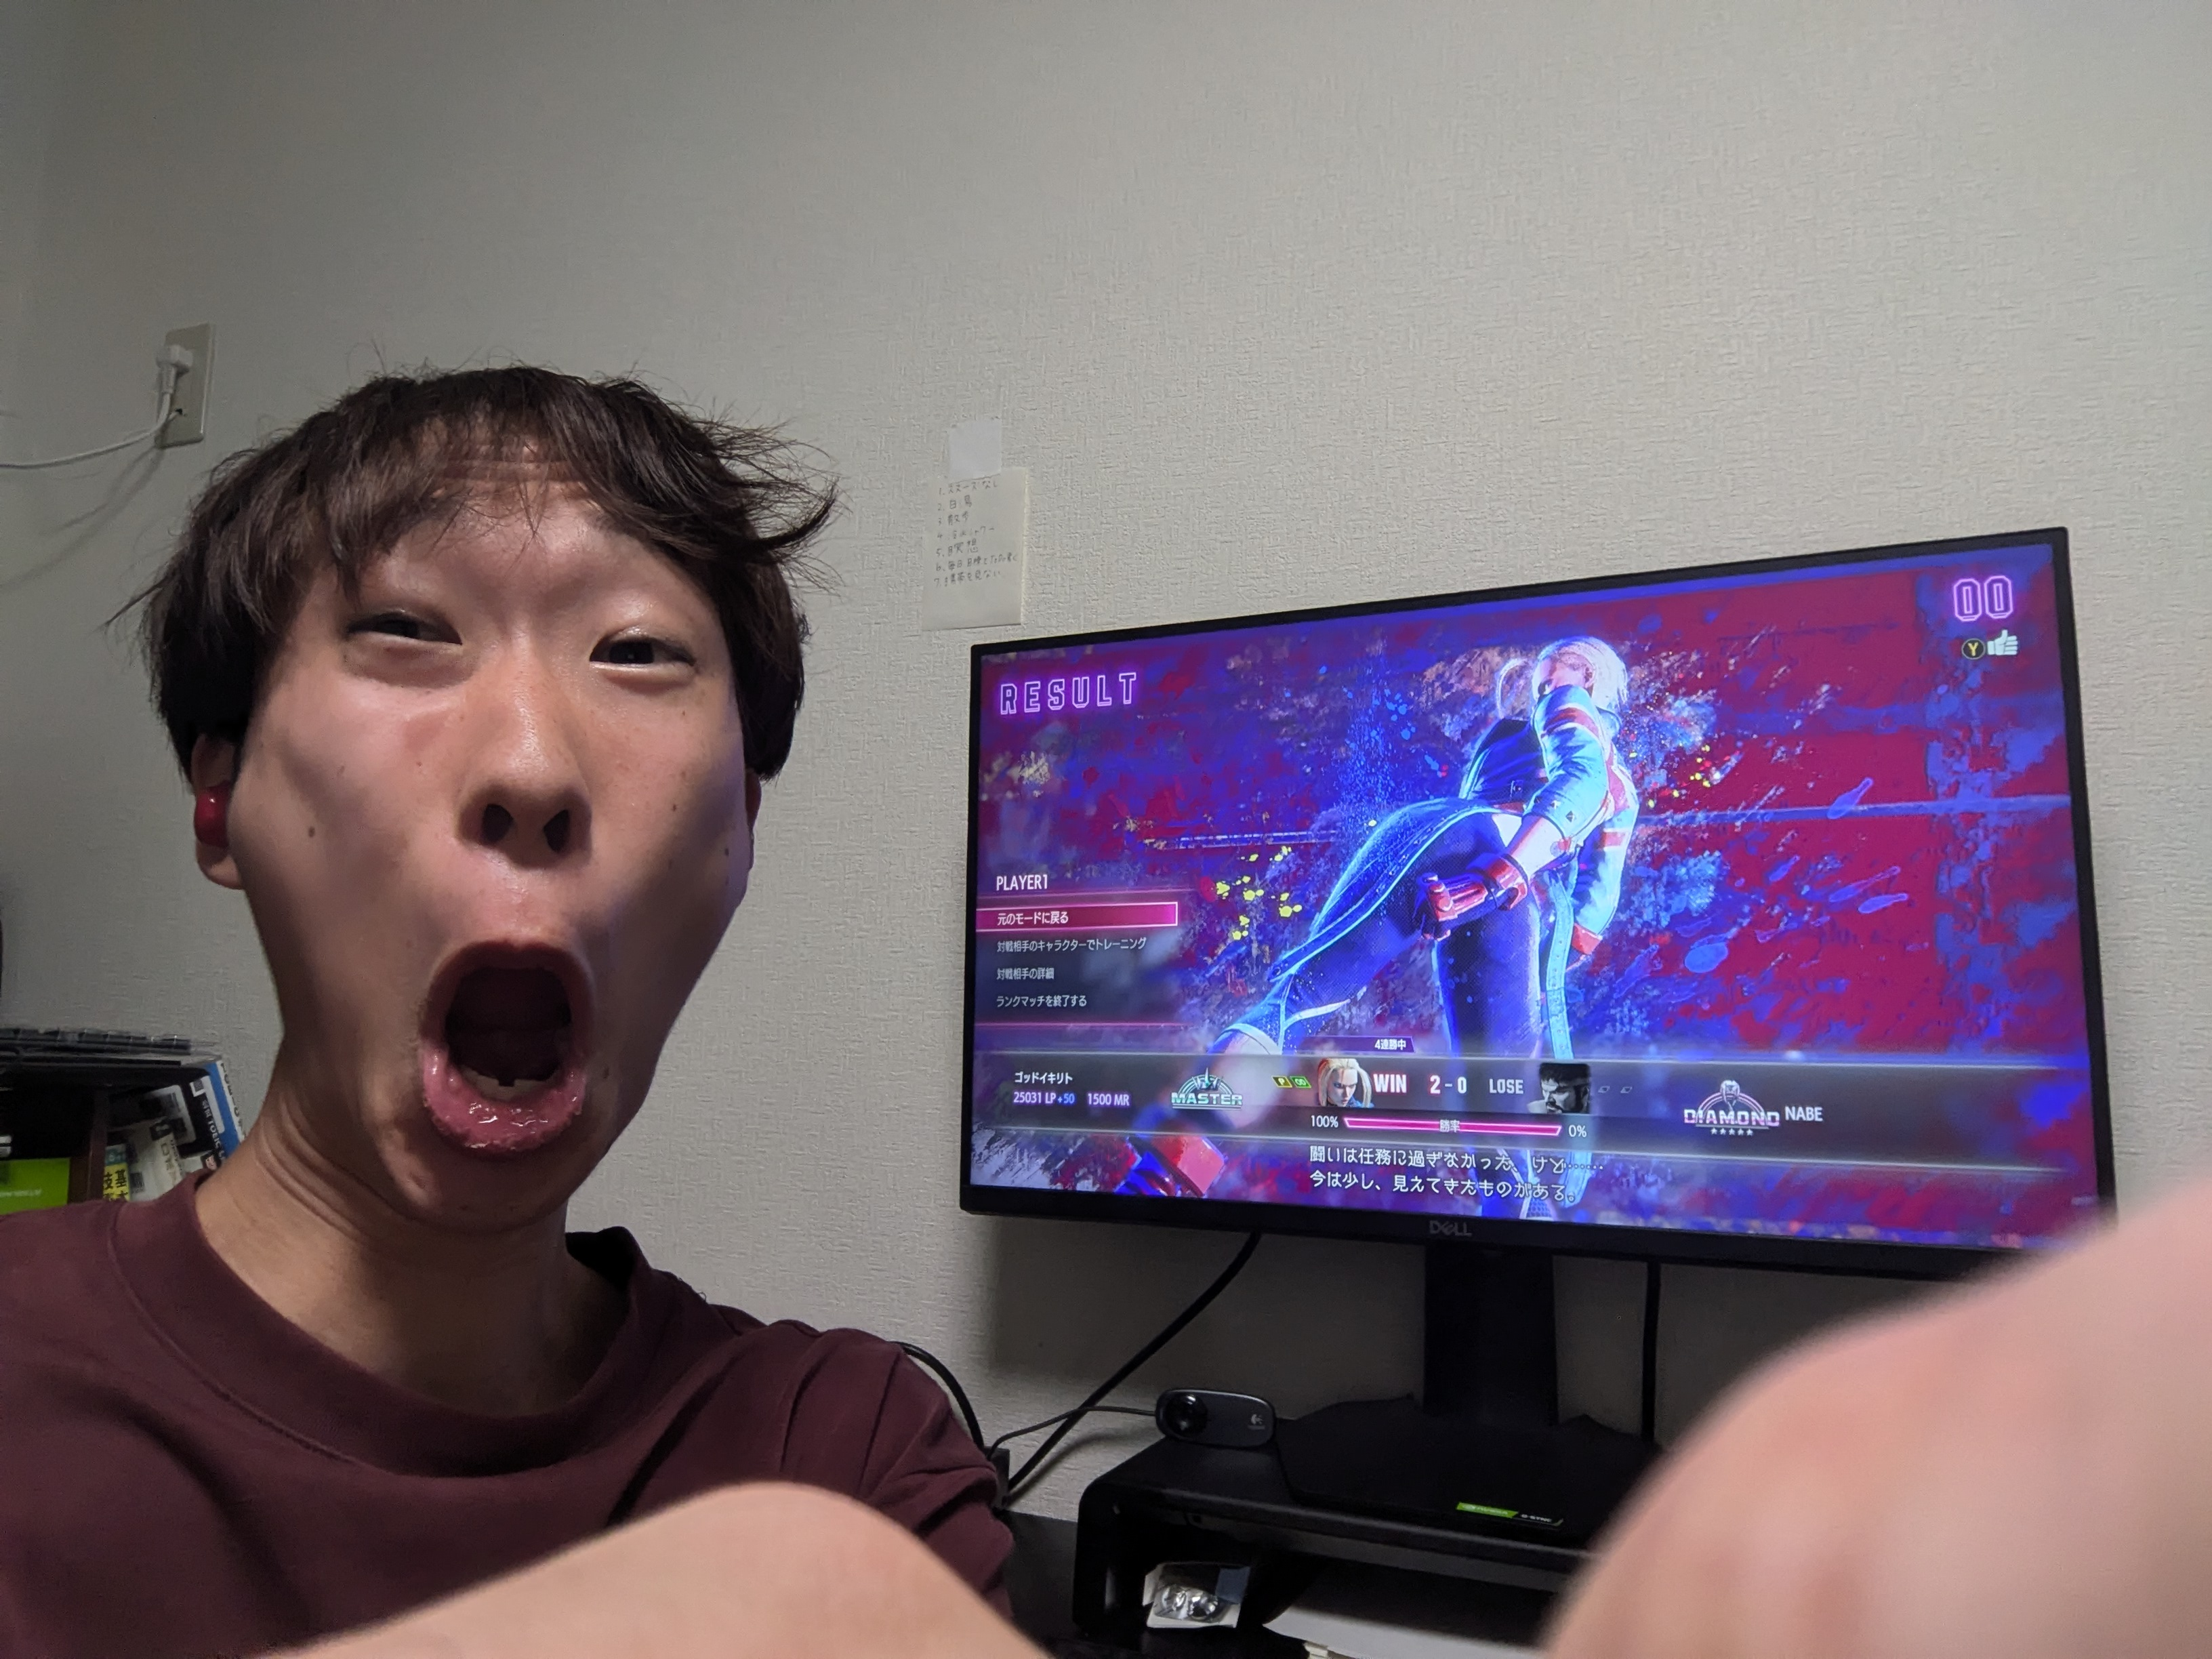
\includegraphics[width=\columnwidth]{img/SF6_Master.jpg}
  \caption{初めてマスターに到達した際の筆者の自撮り写真}\label{fig:sf6_master}
\end{figure}


%----------------------------------------------------------------------------------------------------------
\section{ストリートファイターとは?}
\subsection{シリーズの歴史}
「ストリートファイター」は1987年にアーケードゲームとして登場して以来,対戦格闘ゲームというジャンルを確立し,牽引してきたシリーズである.
その主な歴史は以下の通りである\cite{cite:sf_history}.
\begin{figure}[t]
  \centering
  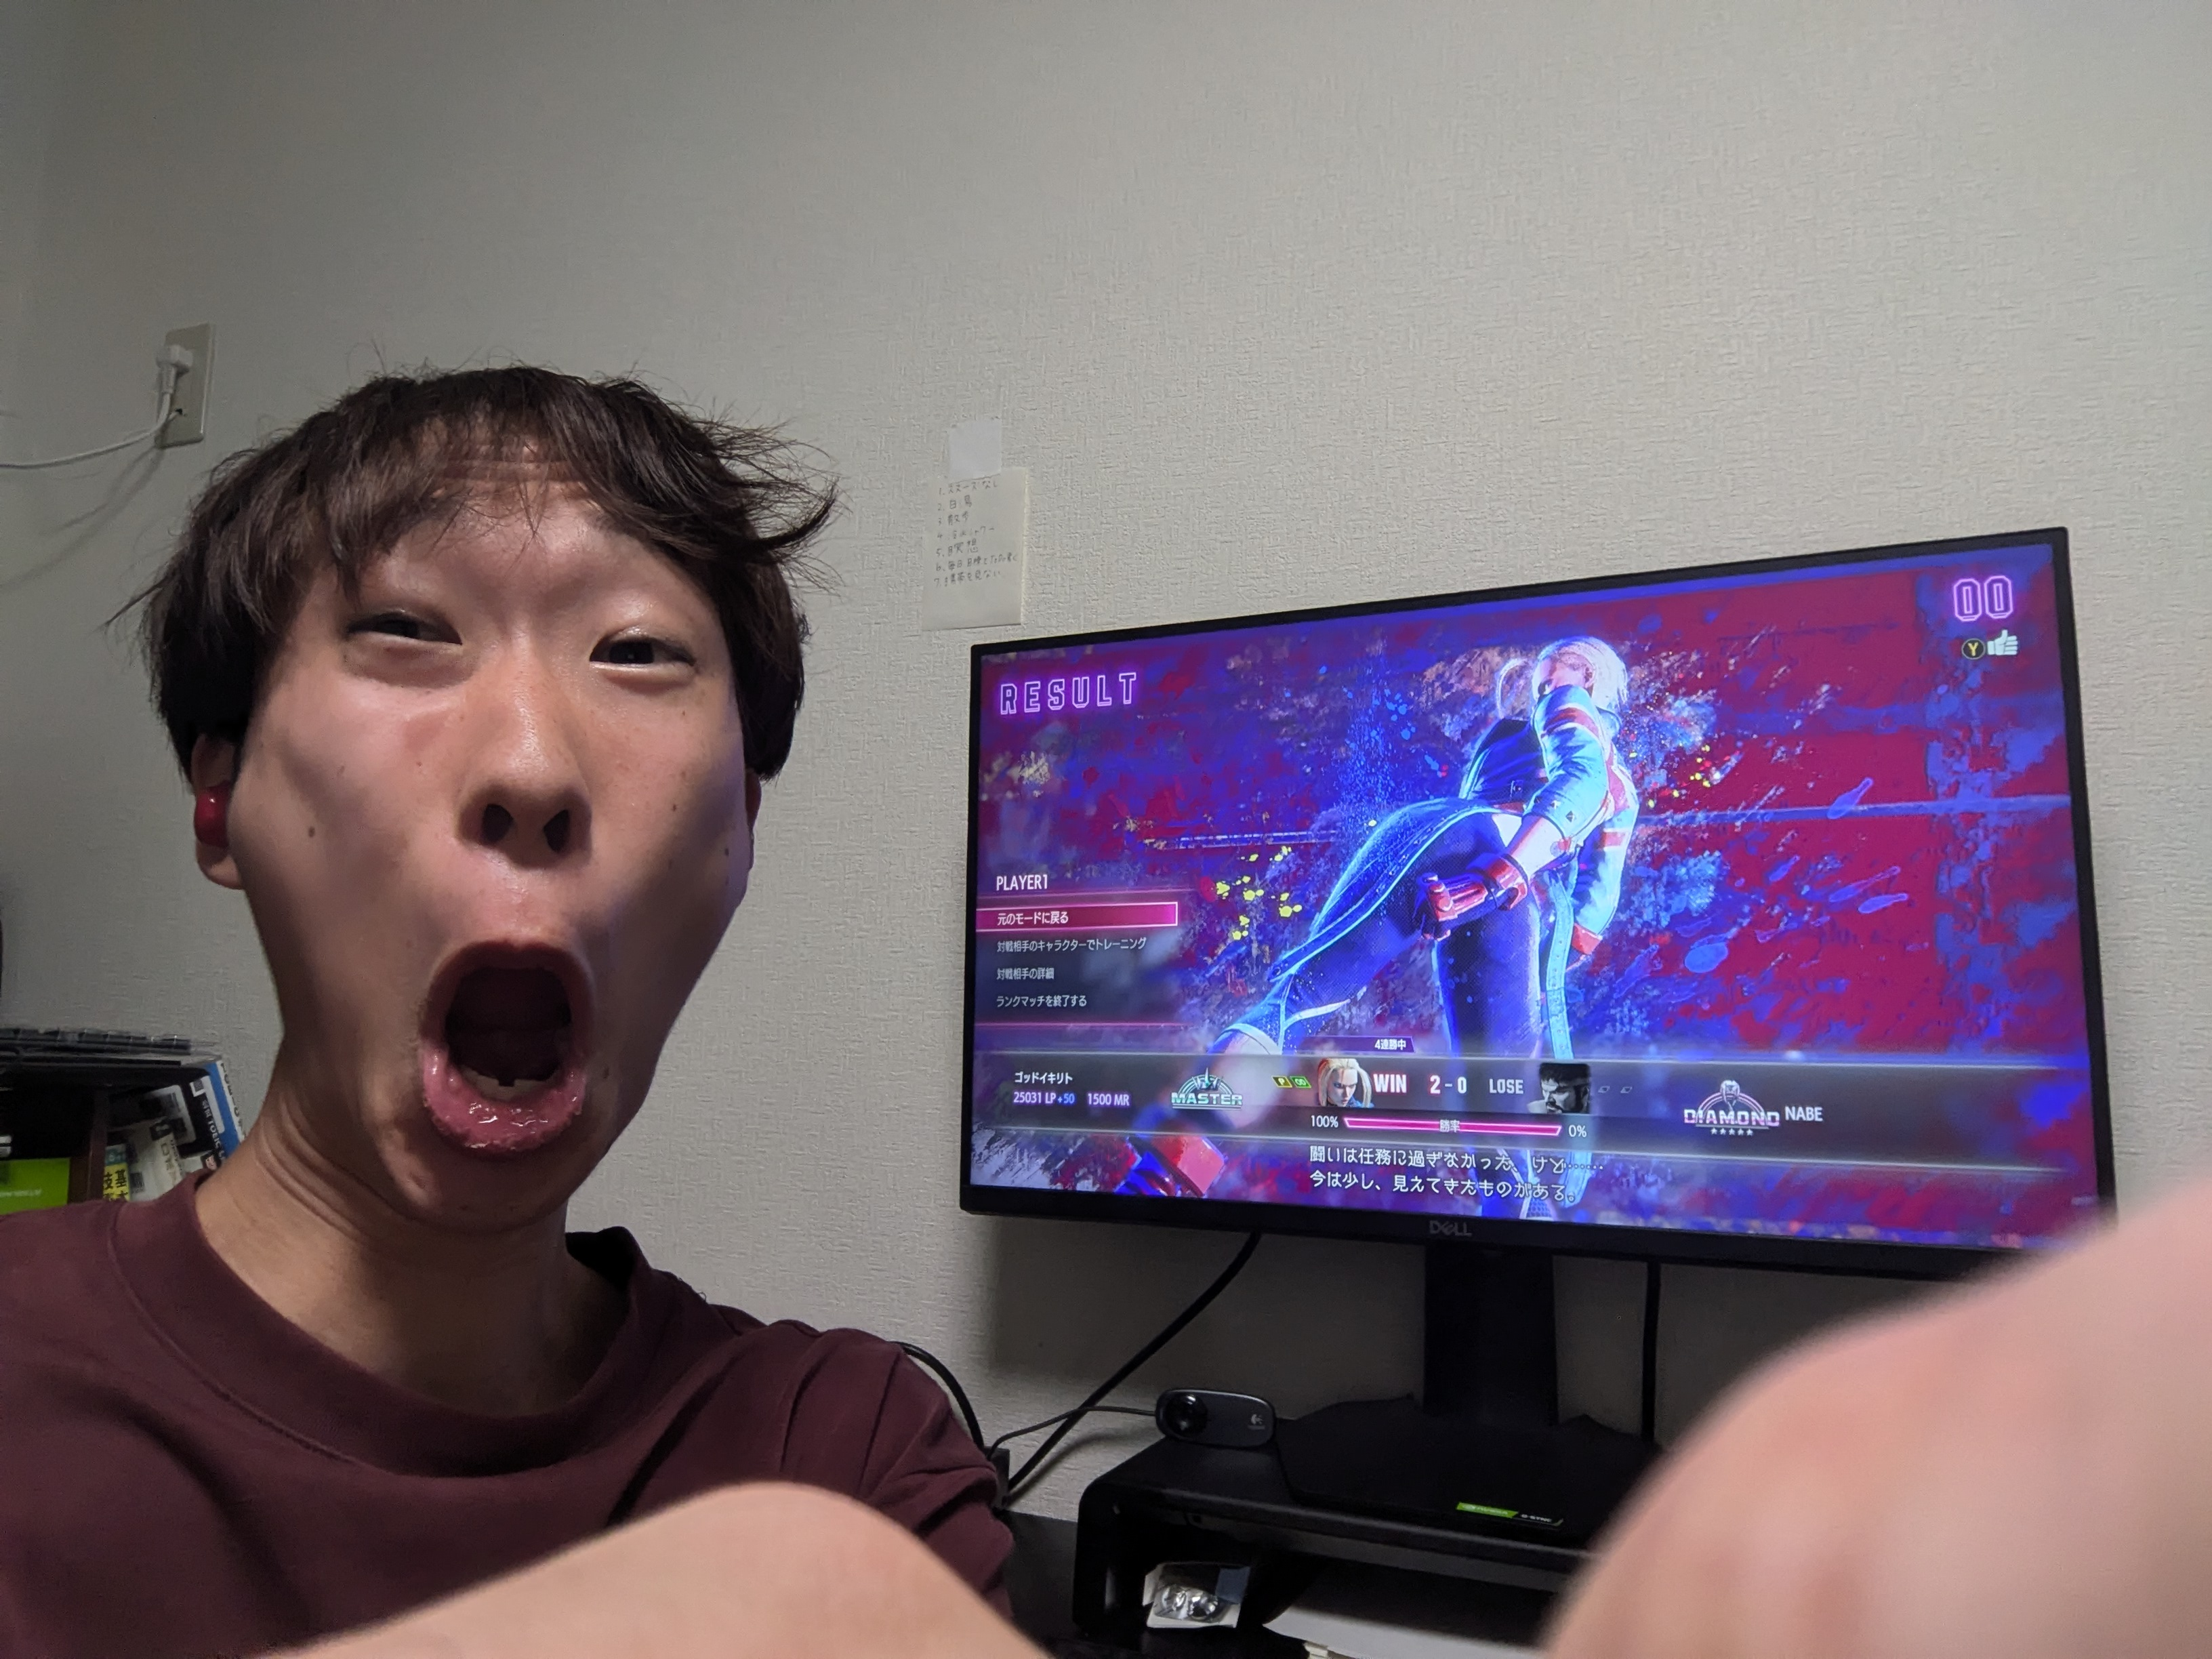
\includegraphics[width=\columnwidth]{img/SF6_Master.jpg}
  \caption{ストリートファイターシリーズ}\label{fig:sf6_master}
\end{figure}
\begin{itemize}
    \item \textbf{ストリートファイターII} (1991年)
    \item \textbf{ストリートファイターZERO} (1995年)
    \item \textbf{ストリートファイターIII} (1997年)
    \item \textbf{ストリートファイターIV} (2008年)
    \item \textbf{ストリートファイターV} (2016年)
    \item \textbf{ストリートファイター6} (2023年)
\end{itemize}
特に1991年の『ストリートファイターII』は社会現象を巻き起こし,2023年の最新作『ストリートファイター6』は世界的なEスポーツシーンの中核を担っている.

\subsection{格闘ゲームの面白さ}
格闘ゲームの試合において、開幕時、劣勢時、優勢時、決着時、その他、いろいろな場面がある。
そのときに「できること」行動の多様さと、その選択が楽しさであると感じる。
場面に応じて相手を観察し、自分の記憶と知識から行動リストを展開し、最適な手を選択する。飛び込み、対空、牽制、突進、めくり、起き上がり、切り返し、そのタイトル固有のシステムなど。
コンボであったり、判定の強さ(判定枠の大きさ)だったり、動きや見た目が好みの技だったり、
その「できること」を(事前にも、戦闘中にも)、調べる、考える、列挙するのは「面白さ」であると思う。

\begin{figure}[t]
  \centering
  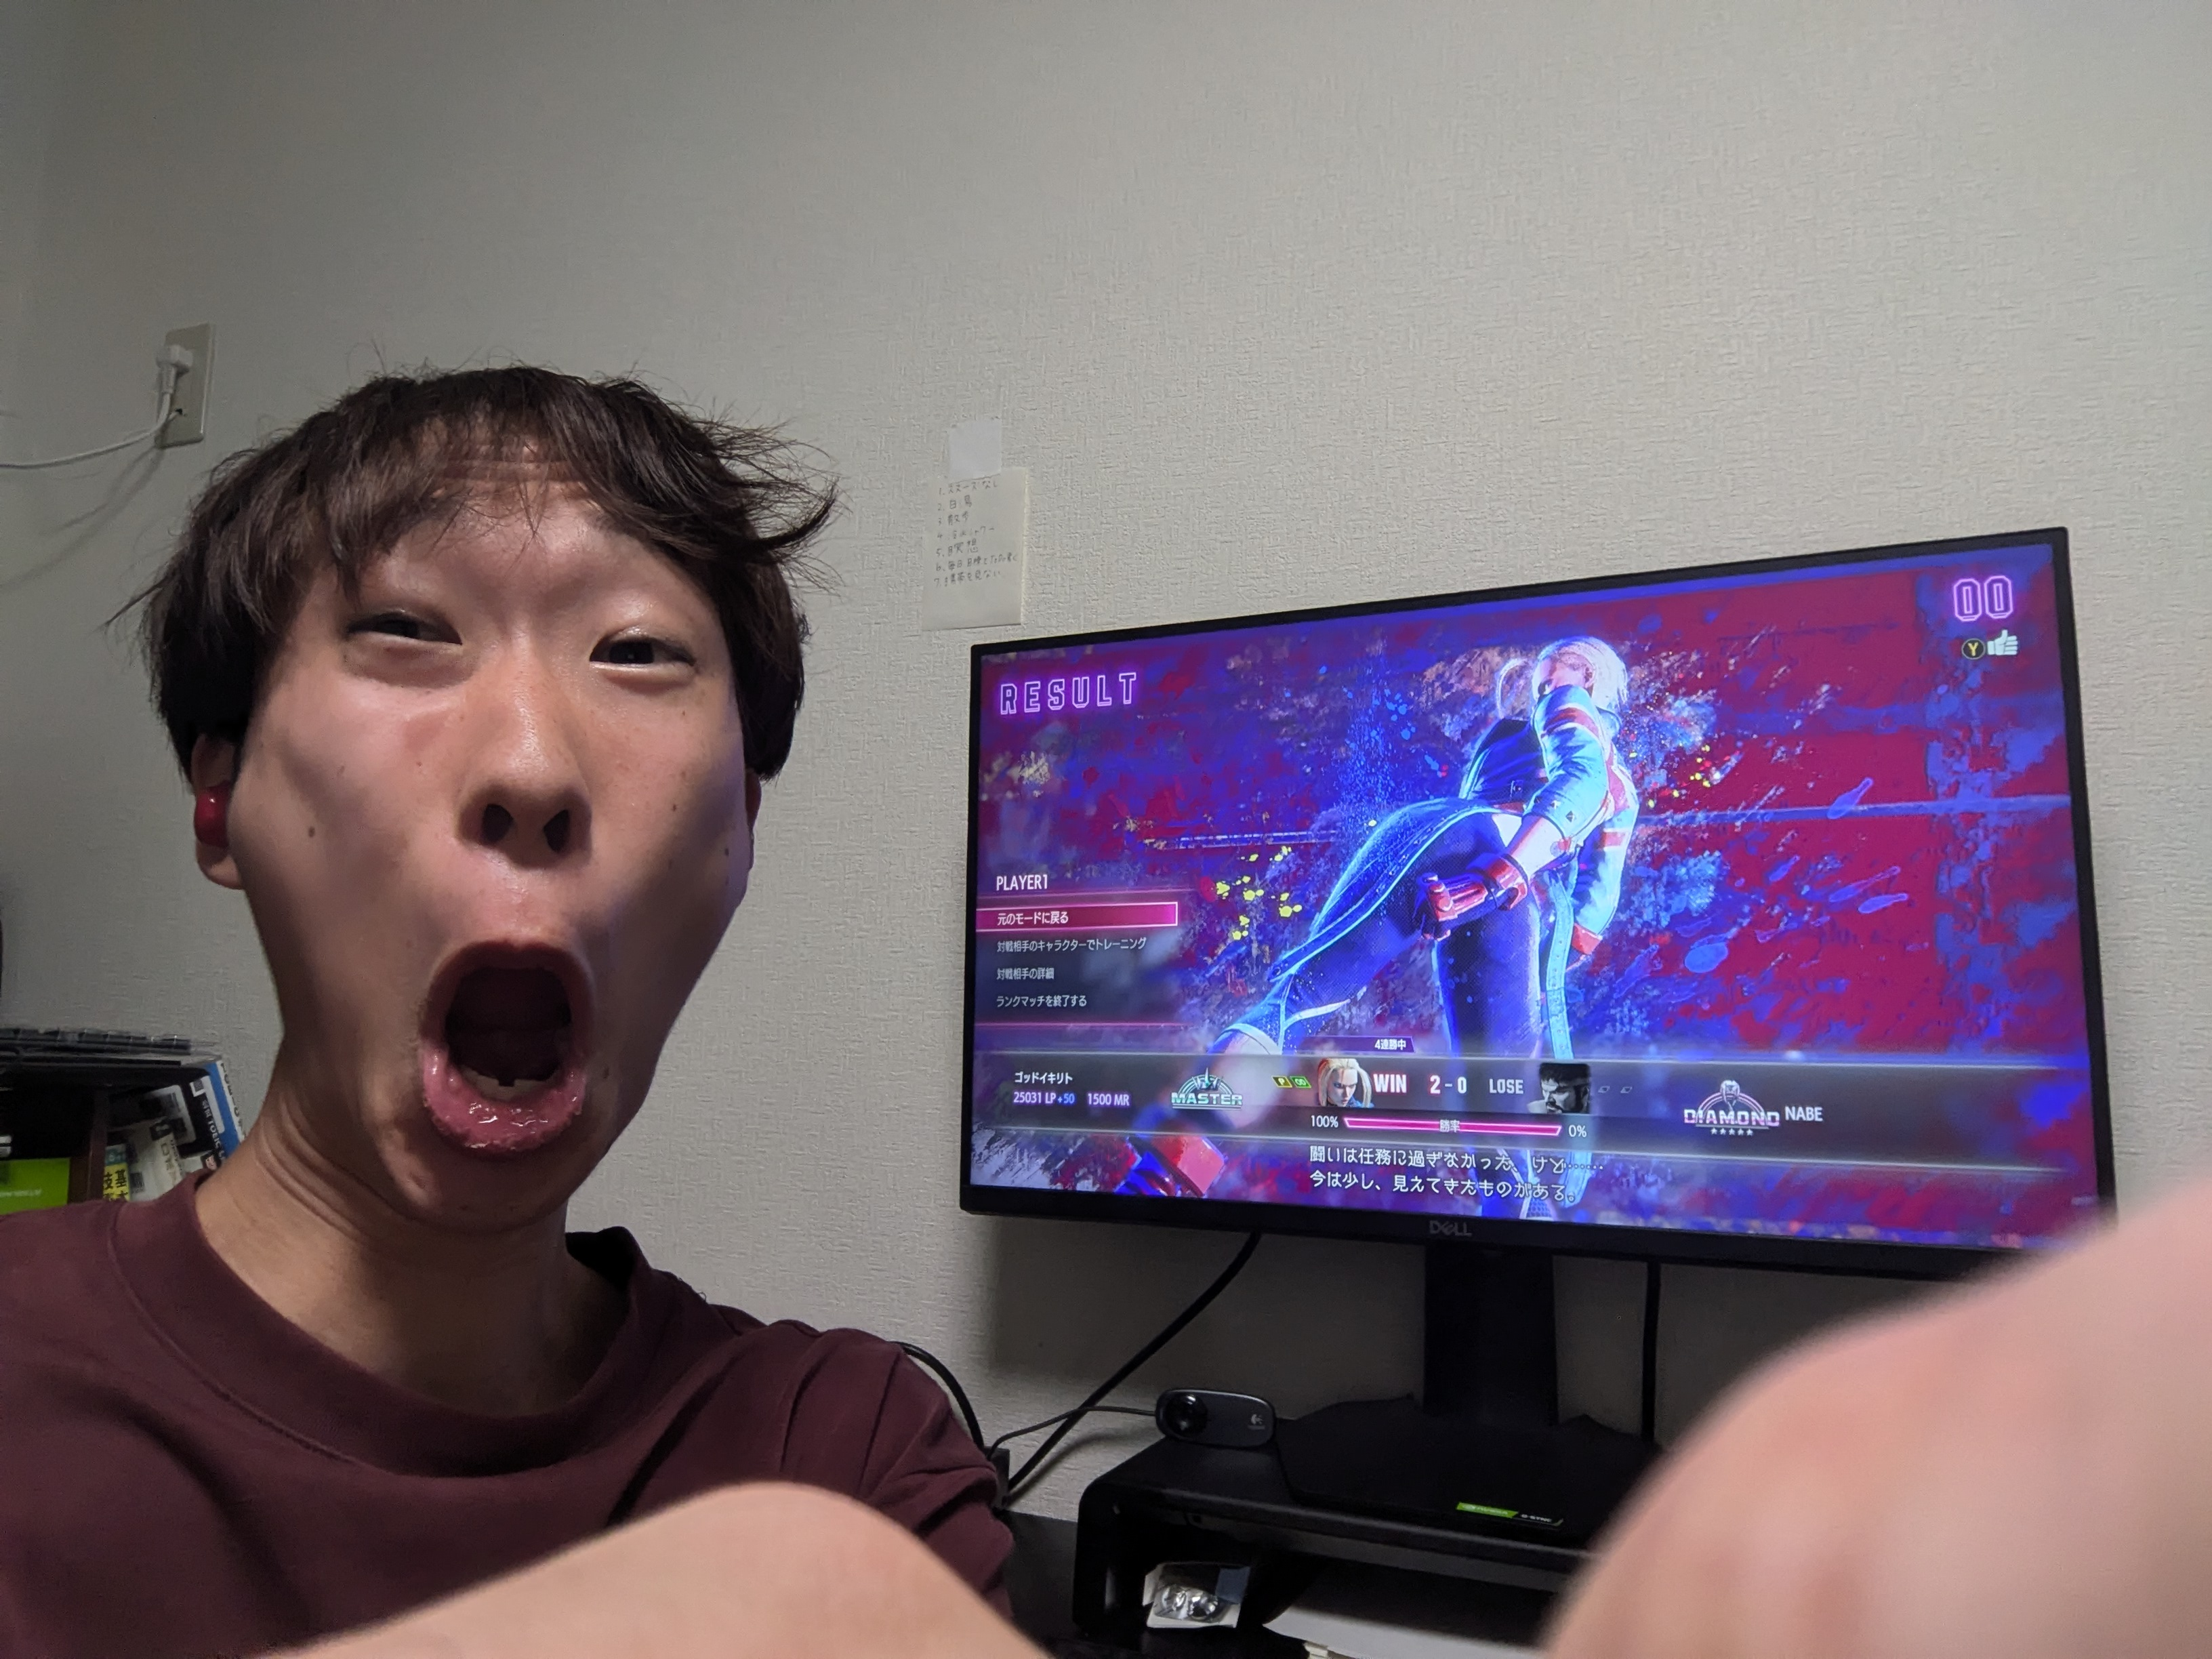
\includegraphics[width=\columnwidth]{img/SF6_Master.jpg}
  \caption{ストリートファイター6 プレイ画面}\label{fig:sf6_master}
\end{figure}

%----------------------------------------------------------------------------------------------------------
\section{ストリートファイターとEスポーツ}
ストリートファイターの競技シーンは,ゲームセンターでの対戦から,世界的なプロツアーへと進化を遂げた.

\subsection{黎明期(1990年〜2000年代)}
1990年代の熱狂はゲームセンターが中心であり,公式な世界大会は存在しなかった.
競技シーンの礎となったのは,現在も世界最大の格闘ゲーム大会である「Evolution Championship Series (EVO)」である.
当初は有志による小規模な大会で,賞金も参加者のエントリー費から賄われる程度であった.

\subsection{転換期(2008年〜)}
『ストリートファイターIV』の登場とオンライン対戦の普及は,大会の規模を国際的なものへと押し上げた.
例えば,EVO 2016のストリートファイターV部門では,参加者5000人以上を集め,賞金総額も10万ドルを超えた\cite{cite:evo2016}.

\subsection{確立期と賞金の高騰(2014年〜)}
2014年,メーカー主催の公式世界ツアー「CAPCOM Pro Tour (CPT)」が設立され,シーンのプロ化が加速した.
当初,年間決勝大会である「CAPCOM CUP 2015」の賞金総額は25万ドルであった\cite{cite:capcomcup_history}.
しかし,シーンの拡大に伴い賞金は高騰.
最新作『ストリートファイター6』を採用した「CAPCOM CUP XI」(2025年3月開催)では,優勝賞金だけで100万ドル(約1.5億円)という破格の金額が設定された\cite{cite:capcom_million}.


\section{ストリートファイター6の始め方}
% TODO ここにSteamでの値段、コントローラー、コマンド、モダン、クラシックについて記載する
PCでプレイする場合、Steamで約5000円で購入。
Switch2, PS5でも同値段でプレイ可能である。

\subsection{コントローラーの選択}
格闘ゲームの操作デバイスには主に3つの選択肢があり,それぞれに特徴がある.
\begin{itemize}
    \item \textbf{アーケードスティック(アケコン)} \\
    ゲームセンターの筐体と同じ感覚でプレイできるコントローラー.左手でレバーを操作し,右手で配置された大きなボタンを押す.直感的な操作が可能で,プロプレイヤーにも愛用者が多い.ただし,サイズが大きく高価な傾向がある.

    \item \textbf{ゲームパッド} \\
    PlayStationやXboxに付属するような一般的なコントローラー.十字キーやアナログスティックでキャラクターを操作する.家庭用ゲーム機に慣れ親しんだプレイヤーにとっては最も手軽に始められる選択肢である.小型で持ち運びやすいが,複雑なコマンド入力には慣れが必要な場合がある.

    \item \textbf{レバーレスコントローラー} \\
    移動も全てボタンで行う,最新型のコントローラー.左手の指で押す移動ボタンにより,レバー操作よりも速く正確な入力が可能とされる.特に防御や必殺技コマンドの入力で有利な場面が多いが,操作感覚が特殊なため,習熟には最も練習が必要となる.
\end{itemize}

初心者はまず手持ちのゲームパッドで試し,より本格的にプレイしたくなった際に他のコントローラーを検討するのが良いだろう.

\begin{figure}[t]
  \centering
  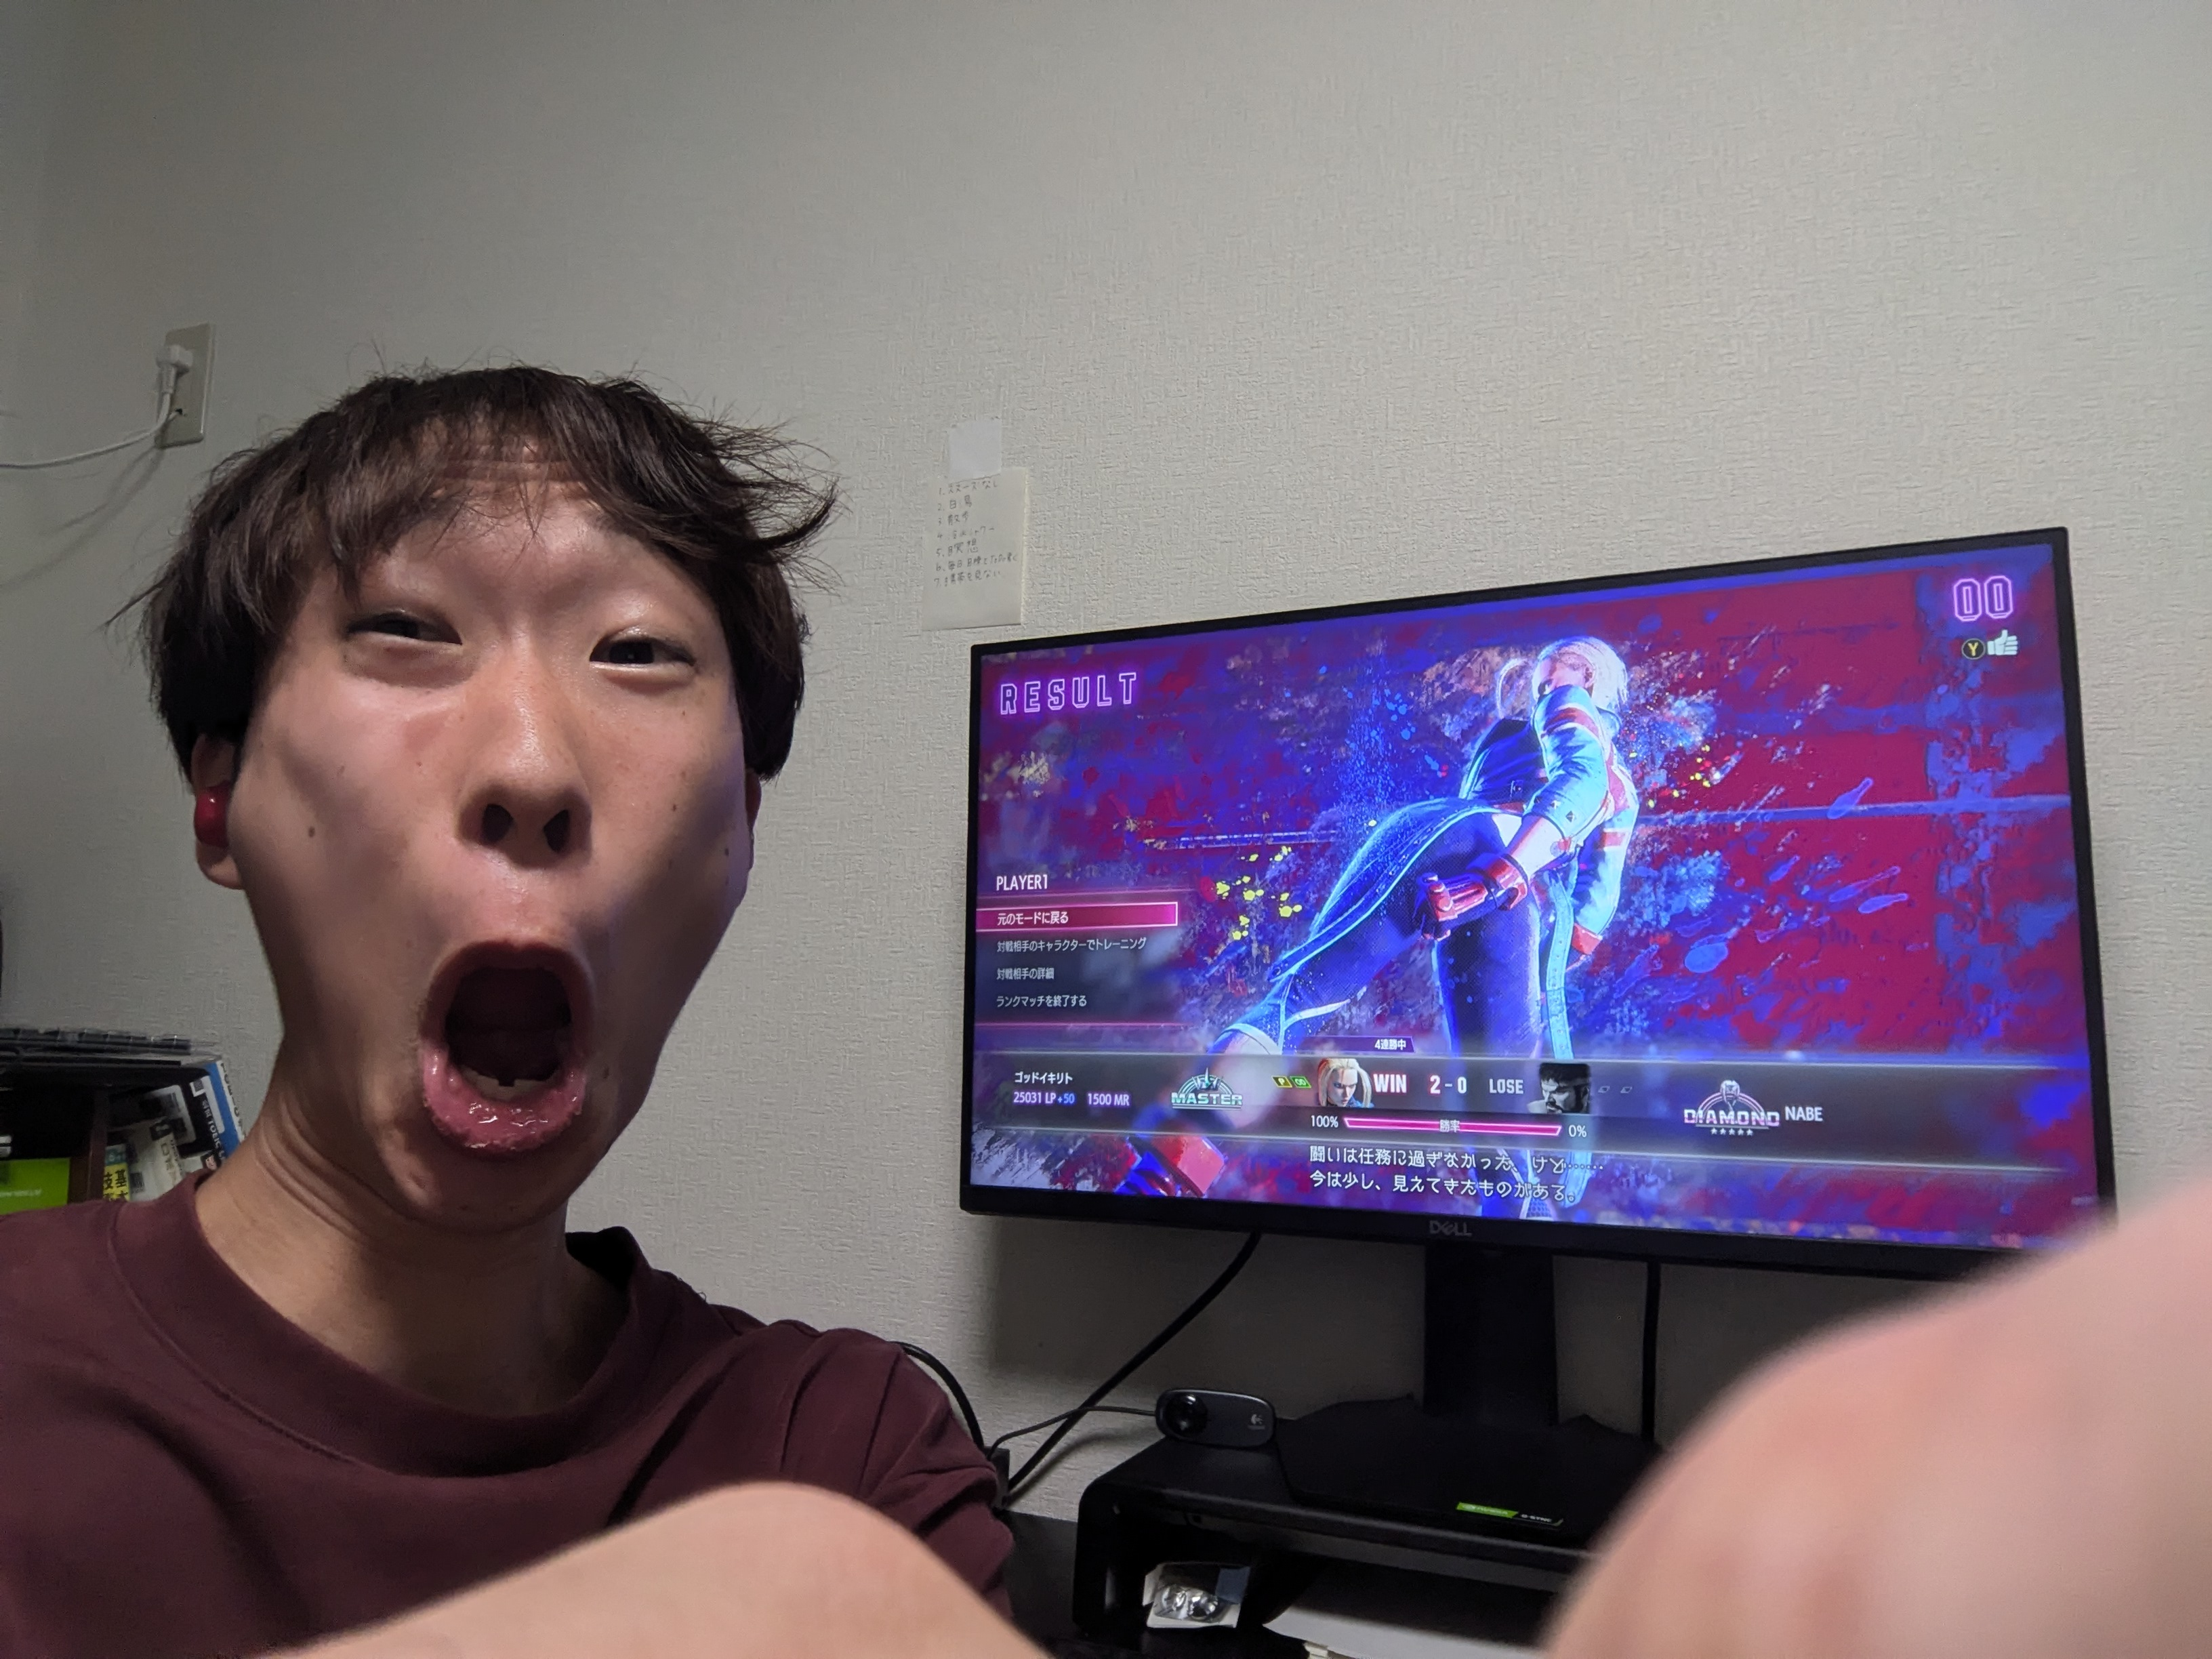
\includegraphics[width=\columnwidth]{img/SF6_Master.jpg}
  \caption{各コントローラーの外見}\label{fig:sf6_master}
\end{figure}

\begin{figure}[t]
  \centering
  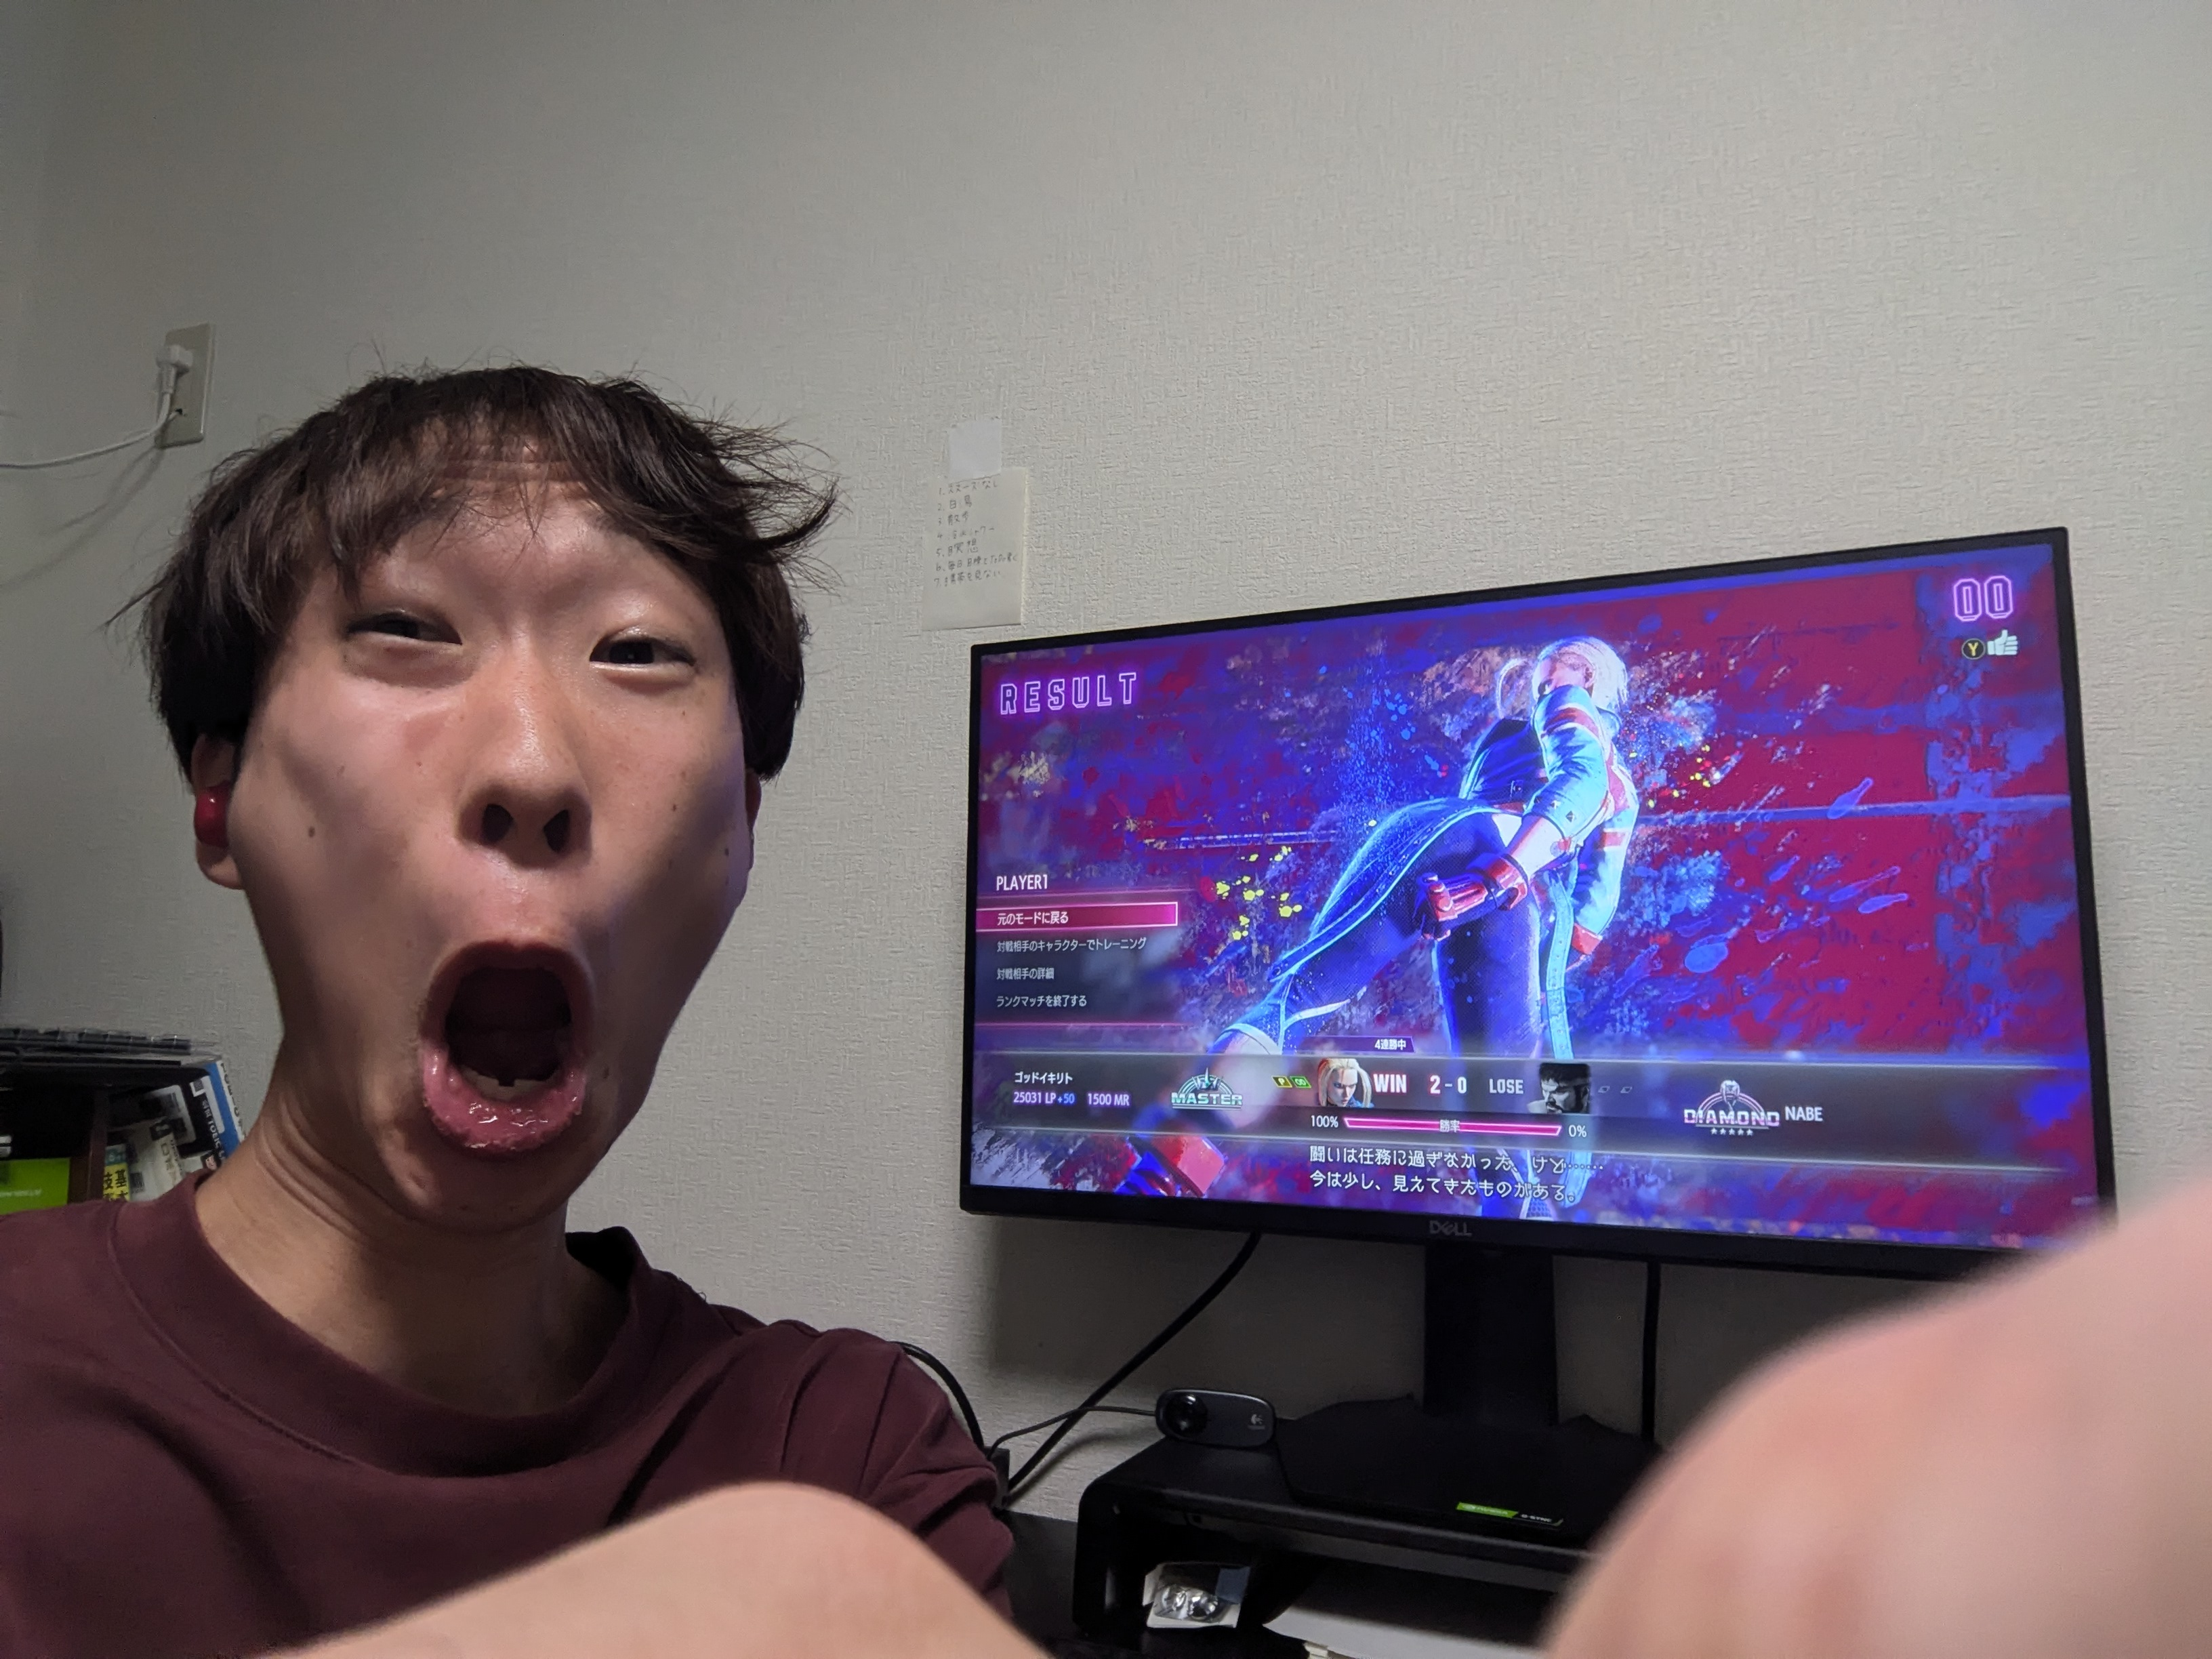
\includegraphics[width=\columnwidth]{img/SF6_Master.jpg}
  \caption{モダンとクラシック}\label{fig:sf6_master}
\end{figure}


\subsection{操作タイプの選択:モダンとクラシック}
『ストリートファイター6』では,プレイヤーの習熟度に合わせて2種類の操作タイプが用意されている.

\subsubsection{モダンタイプ}
必殺技がワンボタンで出せる,初心者に向けたシンプルな操作方法.「アシストボタン」と攻撃ボタンを組み合わせることで,複雑なコンボ(連続技)も簡単に出すことができる.
格闘ゲームの難しい操作を気にすることなく,すぐにキャラクターを動かす楽しさや,相手との読み合いといった戦略的な面白さを体験できるのが最大の利点である.
マスターランクに到達した筆者も,基本モダンタイプを使用している。

\subsubsection{クラシックタイプ}
シリーズ伝統の操作方法.方向キーと6つの攻撃ボタンを組み合わせてキャラクターを操作する.必殺技を出すには「↓ ↘ → + パンチ」のようなコマンド入力が必要となる.
操作の習熟は難しいが,全ての通常技を使い分けることができ,状況に応じた最大限のダメージを与えることが可能.
競技シーンのプレイヤーは,こちらのクラシックタイプを使用していることが多い.

%----------------------------------------------------------------------------------------------------------

\section{まとめ}
筆者はスポーツとEスポーツは本質的に大きく違う、と思っている. 今でこそEスポーツの賞金はとんでもない金額になり, またスポンサー契約などによって
多額の収入を得る選手は少なくない. しかし, たった10年前まではゲームに夢中になること、のめり込むこと自体が否定的にみられ、悪い風潮にあった.
そんな中でも自分が好きなことを貫き通した選手達の価値観や思考はものすごく面白いと筆者は感じている.
Eスポーツはここ10年でものすごく盛り上がってきた業界であるため、試合や大会は面白いのだが、なかでも選手の人間性が魅力だと感じている。
ゲームばかりやって華やかな人生を送ってきていない人もいるが、自分の好きを追求してきた考えや哲学には非常に人生の知見が詰まっている。

%----------------------------------------------------------------------------------------------------------
{\small
\bibliographystyle{jplain}
\bibliography{template}
}
\end{document}